\documentclass{article}
\usepackage{graphicx}
\usepackage[margin=1in]{geometry}
\usepackage{amsmath}
\usepackage{fancyvrb}
\usepackage{float} % Add this package to control figure placement more strictly

\title{Problem Set 6 - Questions 3, 4 and 5}
\author{Yeganeh Karbalaei}
\date{}
\begin{document}
\maketitle
\section{Question 3: Cleaning Dataset}
I used Crimes in U.S communities Dataset from https://www.kaggle.com/:
\begin{itemize}
    \item After installing tidyverse, I used Janitor which makes the process of cleaning easier. I used clean() function to standardize column names and then I looked for missing values. For demographic characteristics, population and income, I set the column median replaces the missing value.  
    \item In next step to make sure that percentage of variables stay in the logical intervals I used the mutate(across()) function. To determine outliers I chose IQR method as Claude suggested me. I set lower boundary as Q1-1.5(Q3-Q1) and upper boundary as Q3+1.5(Q3-Q1). Whatever that has fell between these boundaries is accepted and the rest are outliers. Then, I counted outliers in each column that represented a crime type. 
    \item To remove duplicates I filtered the dataset based on community name, state, county code and community code. I also created income inequality variable to see the inequality between white and black people in each community. 
    \item In last part, the code generates summary statistics, saved cleaned dataset and showed some findings after cleaning process. 
\end{itemize}

\section{Question 4 and 5: Visualization}

\begin{itemize}
    \item I needed a plot to demonstrate ten communities with the highest crime rate and the numbers of the violent crimes, considering the population. At first I checked to see whether there exist a column to show violent crimes per population or not. Then, I asked to sort the 10 communities with high violent crimes descending. After I selected the two variables I needed, in the last step, I created horizontal chart bars.
\end{itemize}

\begin{figure}[H] % Use [H] for "Here absolutely" placement
    \centering
    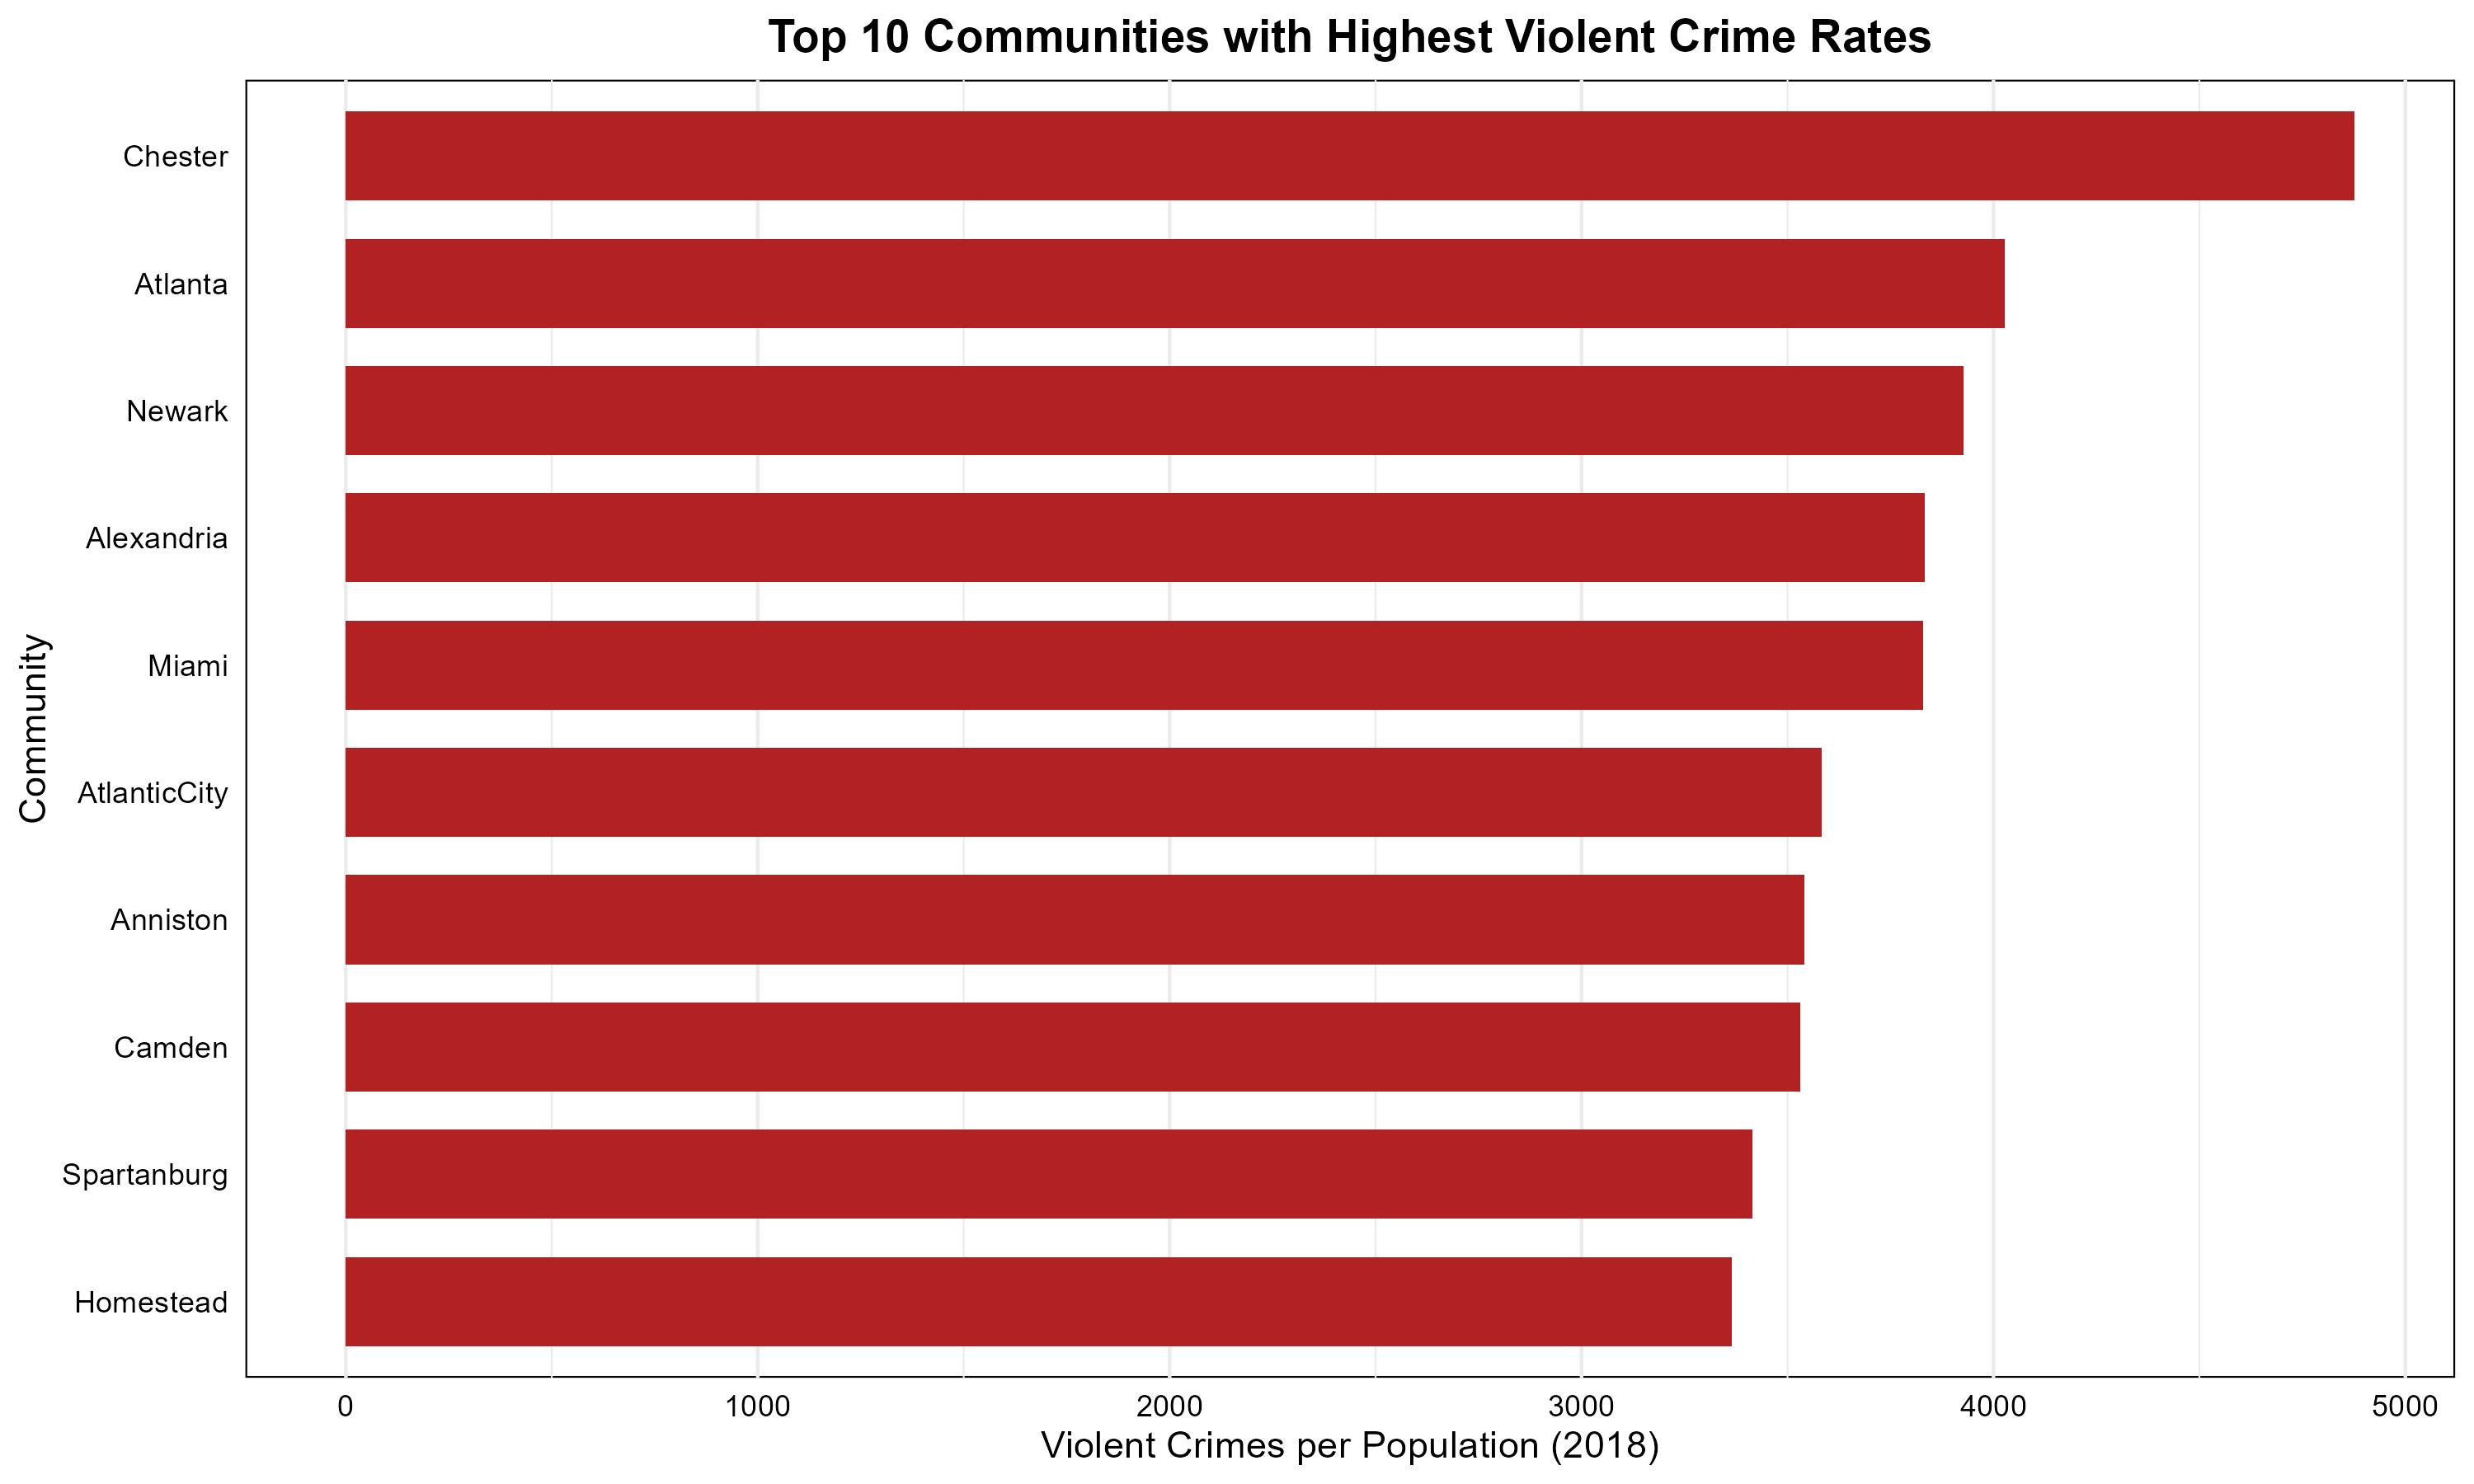
\includegraphics[width=0.8\textwidth]{PS6a_Karbalaei.png}
    \caption{Top 10 Communities with Highest Violent Crime Rates}
    \label{fig:top10communities}
\end{figure}

\begin{itemize}
    \item For second plot, I liked to see whether the communities with high inequality have higher violent crimes rate or not. Hence, I used the income inequality variable that I defined earlier. I selected five communities with highest violent crime numbers and five communities which had non-zero lowest crime rates. As Claud suggested me, I used aes() in order to map data variables to visual properties of the plot. The bars' colors are based on crime leve. Red is for communities with high crima rate and blue for the ones who had lower crime rates. As it is shown we have communities with low inequality but they have high crime rates like Newark. 
\end{itemize}

\begin{figure}[H]
    \centering
    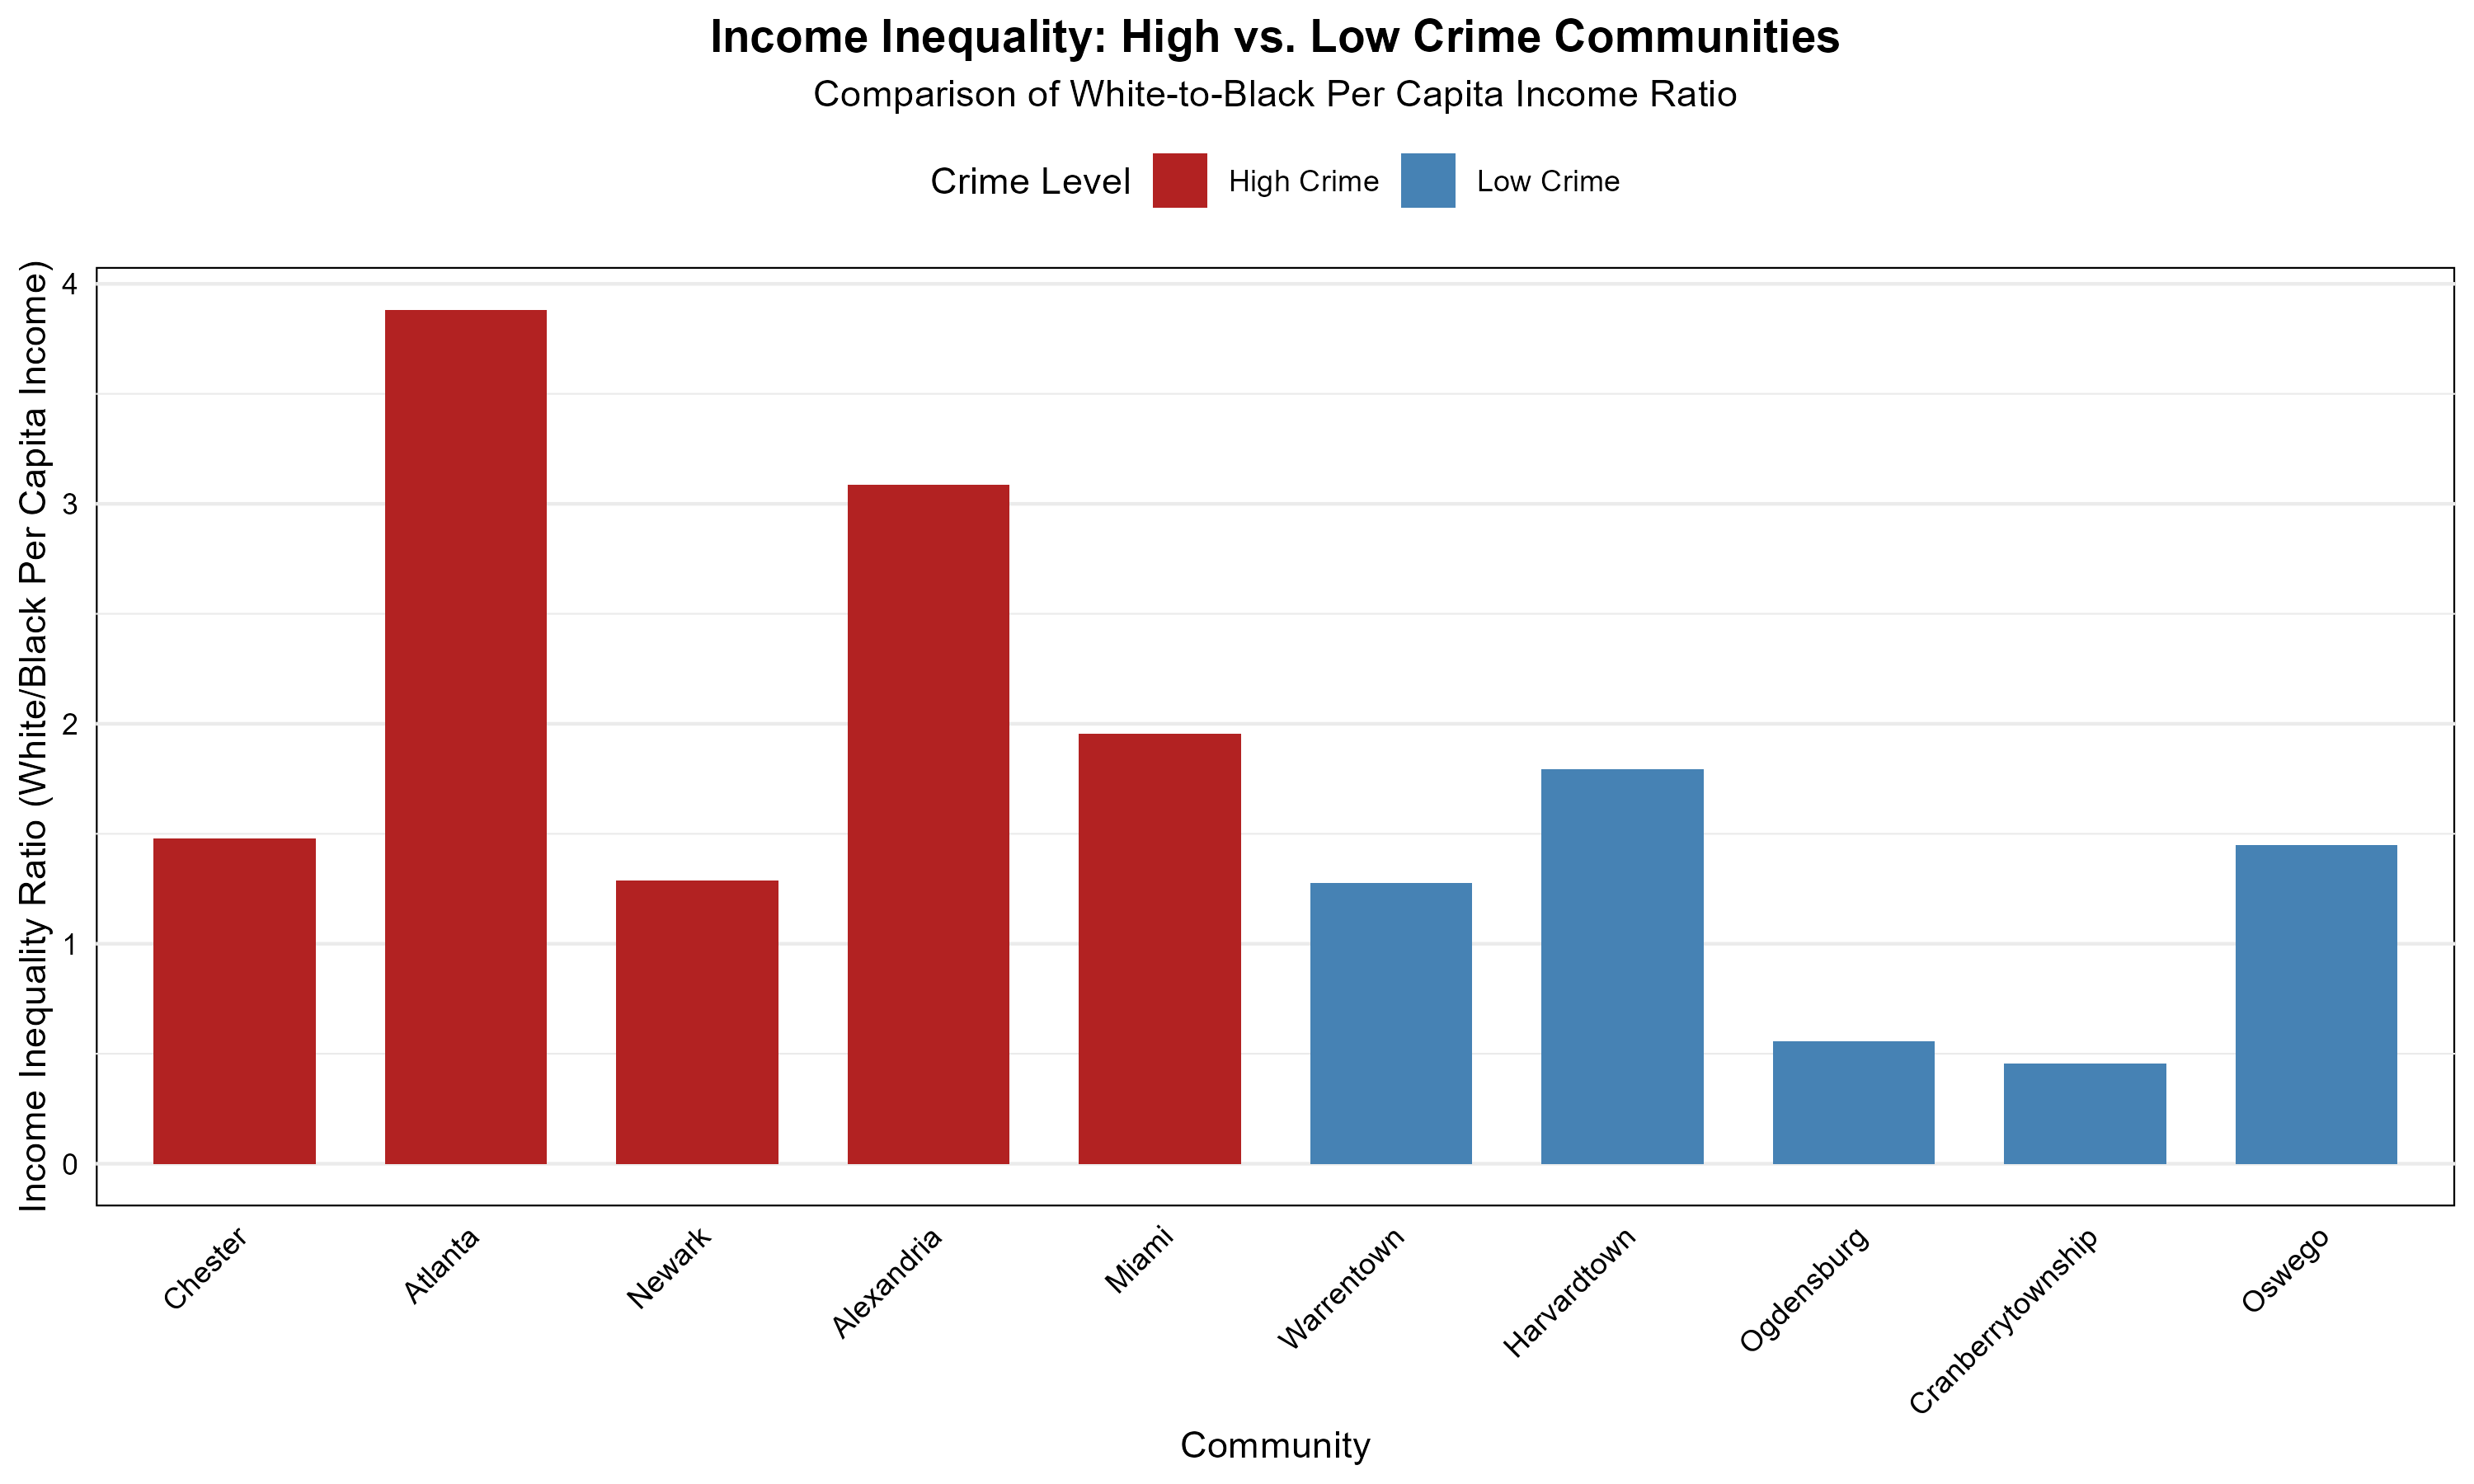
\includegraphics[width=0.8\textwidth]{PS6b_Karbalaei.png}
    \caption{Income Inequality Comparison: High vs. Low Crime Communities}
    \label{fig:inequality}
\end{figure}

\begin{itemize}
    \item In the third plot, I wanted to reorder the communities based on their states to see which states have the most dangerous communities. At first, by using filter(), the states who had less than three communities in dataset were deleted. Then I chose 15 states with their average crime rate. By geomjitter() I created a scatterplot in which the points are shifted in order to avoid overlapping. geomboxplot shows the distribution of data and thememinimal helps the to create cleaner visualization.  
\end{itemize}

\begin{figure}[H]
    \centering
    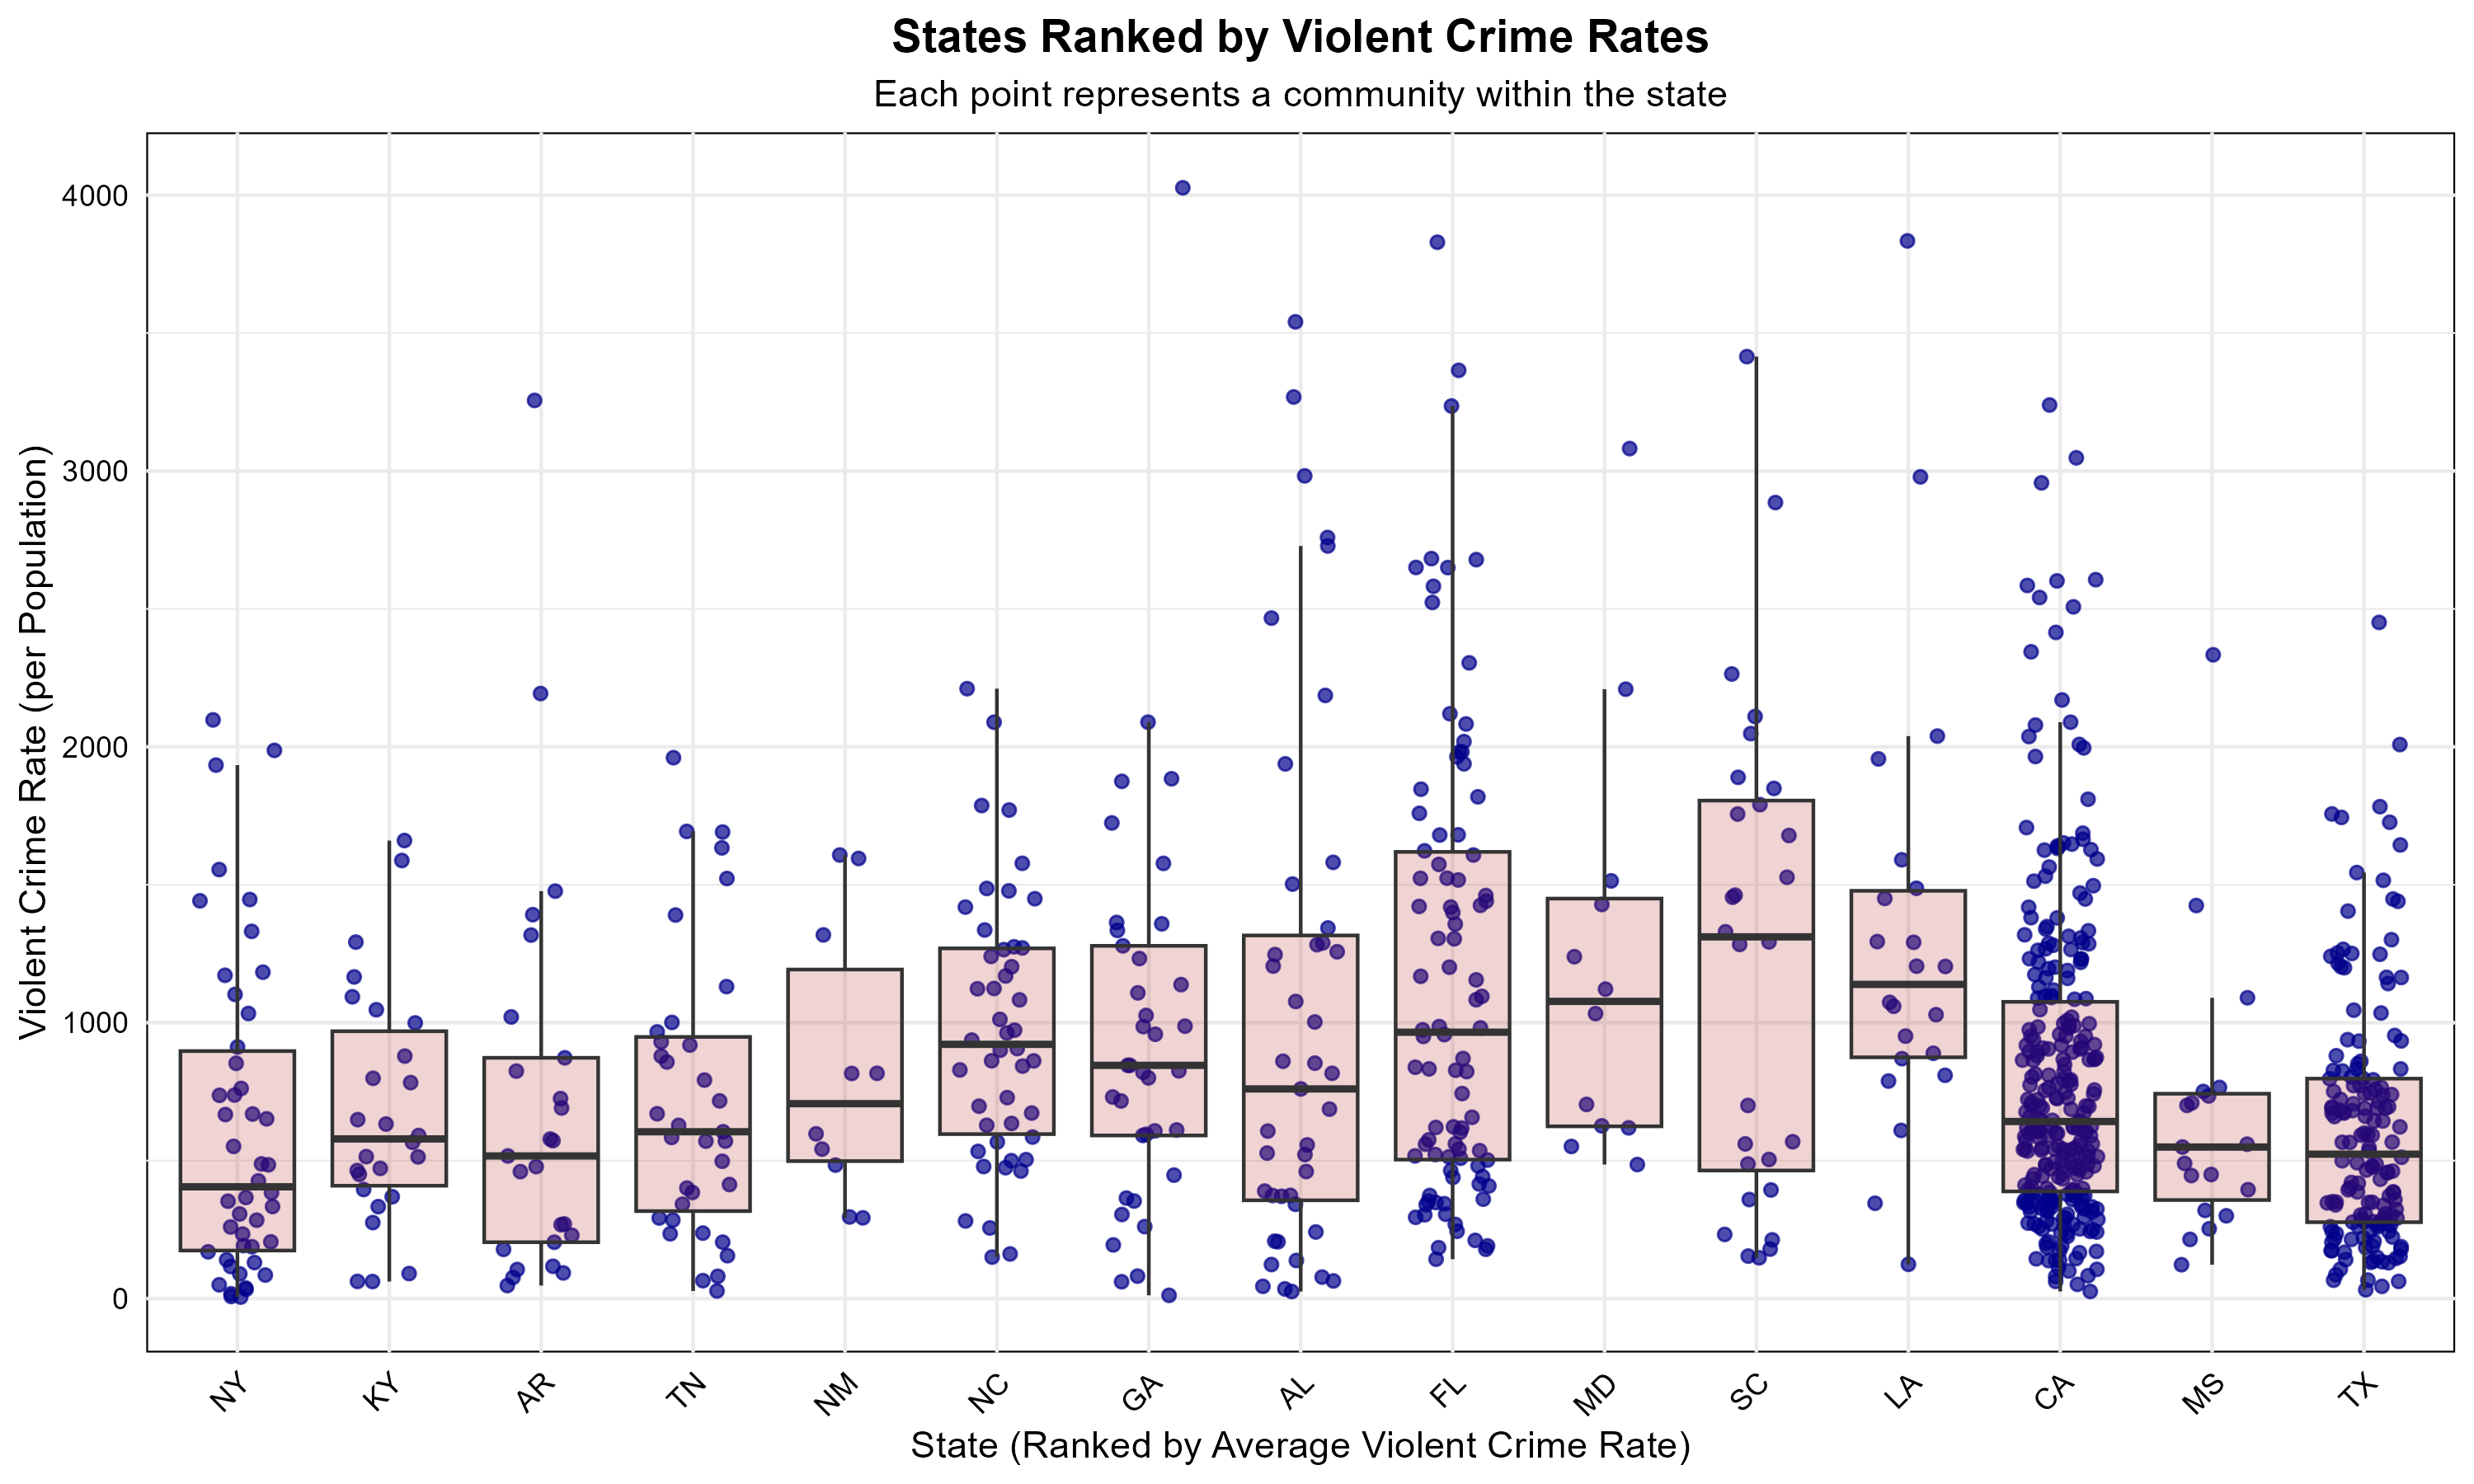
\includegraphics[width=0.8\textwidth]{PS6c_Karbalaei.png}
    \caption{States Ranked by Violent Crime Rates}
    \label{fig:states}
\end{figure}

\end{document}